\documentclass{beamer}
\usepackage{beamerthemesplit}
\usetheme{SPbGU}
%{CambridgeUS}
% Выпишем часть возможных стилей, некоторые из них могут содержать
% дополнительные опции
% Darmstadt, Ilmenau, CambridgeUS, default, Bergen, Madrid, AnnArbor,Pittsburg, Rochester,
% Antiles, Montpellier, Berkley, Berlin
\usepackage{pdfpages}
\usepackage{amsmath}
\usepackage{cmap} % for serchable pdf's
\usepackage[T2A]{fontenc} 
\usepackage[utf8]{inputenc}
\usepackage[english,russian]{babel}
\usepackage{indentfirst}
\usepackage{amsmath}
\usepackage{dot2texi}
\usepackage{tikz}
\usepackage{fancyvrb}
\usepackage{graphicx}
\usepackage{array}
%\usepackage[usenames,dvipsnames]{color}
\usetikzlibrary{shapes,arrows}
% Если у вас есть логотип вашей кафедры, факультета или университета, то
% его можно включить в презентацию.

%\usefoottemplate{\vbox{}}%  \tinycolouredline{structure!25}% {\color{white}\textbf{\insertshortauthor\hfill% \insertshortinstitute}}% \tinycolouredline{structure}% {\color{white}\textbf{\insertshorttitle}\hfill}% }}

%\logo{
\includegraphics[width=1cm]{SPbGU_Logo.png}}

%[GLR-анализатор]
\title[]{Абстрактный синтаксический анализ на основе GLR-алгоритма}
%\subtitle[студроект]{Студенческий проект}
\institute[JetBrains]{
Лаборатория JetBrains на Математико-Механическом факультете \\
Санкт-Петербургского государственного университета }

\author[Григорьев Семён]{Григорьев Семён Вячеславович}

\date{24 октября 2013г.}

\begin{document}

\begin{frame}
    \begin{tabular}[c c c]{m{3cm} m{5.5cm} m{2cm}}
        \begin{center}
        
\includegraphics[width=2.5cm]{JBLogoWhite.png}
    \end{center}
    &
    Девятая независимая научно-практическая конференция \newline "Pазработка ПО 2013" 
    \newline
    23-25 октября, Москва
    &
    \begin{center}
        
\includegraphics[width=2cm]{SecrLogo.png}
    \end{center}
    \\
    &&
    \end{tabular}
    \titlepage
\end{frame}

\definecolor{orange}{RGB}{179,36,31}
\begin{frame}[fragile]
	\transwipe[direction=90]
	\frametitle{Встроенные языки}
	\begin{itemize}
		\item Динамический SQL
		\begin{Verbatim}[commandchars=\\\{\}]
\textcolor{blue}{IF} @X = @Y
    \textcolor{blue}{SET} @TABLE = \textcolor{orange}{'#table1'}
\textcolor{blue}{ELSE}
    \textcolor{blue}{SET} @TABLE = \textcolor{orange}{'table2'}
\textcolor{blue}{EXECUTE} 
    (\textcolor{orange}{'SELECT x FROM'} + @TABLE + \textcolor{orange}{' WHERE ISNULL(n,0) > 1'})
		\end{Verbatim}
		\item JavaScript в Java
		\begin{Verbatim}[commandchars=\\\{\}]
\textcolor{blue}{String} script =
    \textcolor{orange}{"function hello(name) { print(’Hello, ’ + name); }"};
engine.eval(script);
\textcolor{blue}{Invocable} inv = (\textcolor{blue}{Invocable}) engine;
inv.invokeFunction(\textcolor{orange}{"hello"}, \textcolor{orange}{"Scripting!!!"} );
        \end{Verbatim}
	\end{itemize}
\end{frame}

\begin{frame}[fragile]
	\transwipe[direction=90]
	\frametitle{Проблема}
	\begin{itemize}
	    \item Ошибки в динамически формируемых выражениях обнаруживаются лишь во время выполнения.
	    \item Динамически формируемые выражения -- код на некотором языке. Его нужно соответствующим образом поддерживать и обрабатывать.
        \begin{itemize}
	        \item Поддержка в IDE.
	        \item Реинжиниринг ПО, разработанного с использованием встроенных языков.
	    \end{itemize}
    \end{itemize}
\end{frame}

\begin{frame}[fragile]
	\transwipe[direction=90]
	\frametitle{Предлагаемое решение}
	\begin{itemize}
	    \item Статический анализ для встроенных языков. Абстрактный лексический и синтаксический анализы.
	    \begin{itemize}
		    \item Поддержка в IDE:
        	\begin{itemize}
        		\item Многие ошибки можно искать без запуска программы.
            	\item Автодополнение, рефакторинги.
            	\item Возможны трансформации.
            \end{itemize}
	        \item Реинжиниринг:
        	\begin{itemize}
        		\item Статический анализ.
            	\item Трансформация (трансляция).
            \end{itemize}
	    \end{itemize}
    \end{itemize}
\end{frame}

\begin{frame}[fragile]
	\transwipe[direction=90]
	\frametitle{Пример работы}
	\begin{center}
	    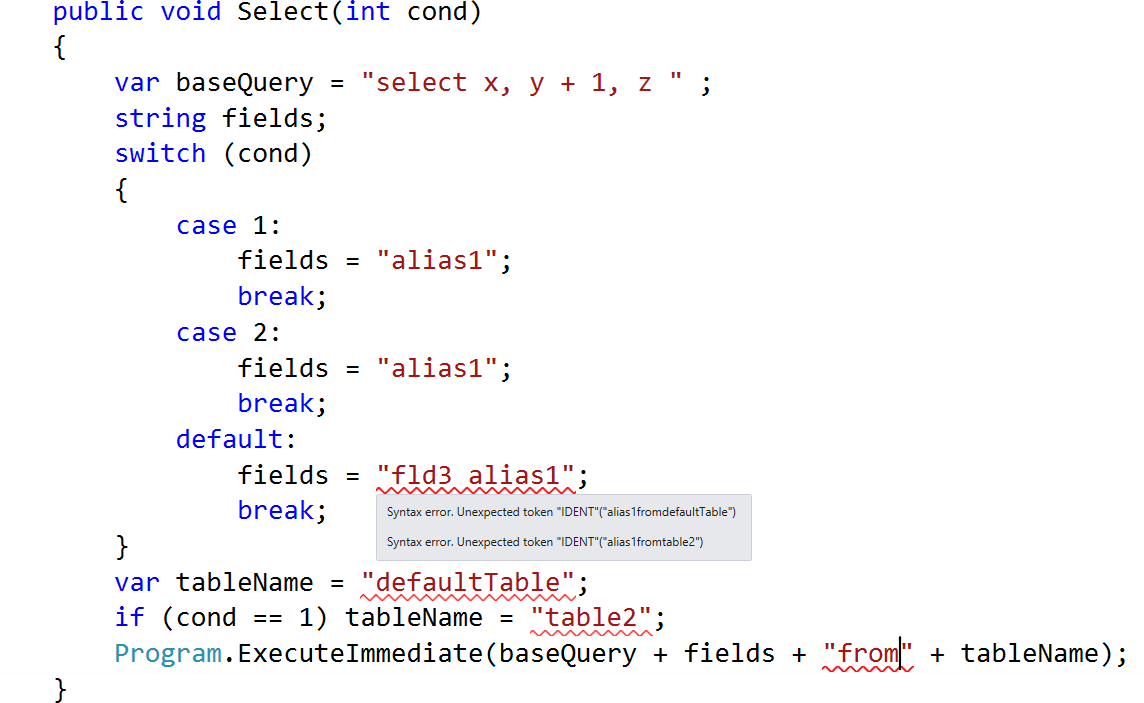
\includegraphics[width=290pt]{Screen1.png}
	\end{center}
\end{frame}

\begin{frame}[fragile]
	\transwipe[direction=90]
	\frametitle{Существующие решения}
	\begin{itemize}
	    \item Alvor -- плагин для Eclipse для статической проверки встоенного в Java SQL.
	    \item Java String Analyzer -- статический анализатор динамических выражеий для Java. 
		\item PHP String Analyzer -- статический анализатор динамических выражеий для PHP.
    \end{itemize}
    В основе этих реализаций лежит (G)LR-анализ и они используют дополнительные структуры данных для организации стека и вычисления семантики.
\end{frame}

\begin{frame}[fragile]
	\transwipe[direction=90]
	\frametitle{Как это работает}
	\begin{itemize}
	    \item Для каждого выражения строится конструкция, аппроксимирующая множество его возможных значений.
    	\begin{itemize}
    		\item Data-flow уравнение
        	\item \textbf{Граф}
        	\item Регулярное выражение
        \end{itemize}
	    \item Выполнение лексического, синтаксического анализа над графом -- абстрактный анализ.
    \end{itemize}
\end{frame}

\begin{frame}[fragile]
	\transwipe[direction=90]
	\frametitle{Пример}
	\begin{itemize}
	    \item Kод:
    	\begin{Verbatim}[commandchars=\\\{\}]
\textcolor{blue}{var} tbl1 = \textcolor{orange}{“#tbl1”} 
\textcolor{blue}{var} tbl2 = \textcolor{orange}{“tbl2”}
\textcolor{blue}{execute} (\textcolor{orange}{“select x from ”} + \textcolor{blue}{if} cond \textcolor{blue}{then} tbl1 \textcolor{blue}{else} tbl2)
        \end{Verbatim}
	    \item Входной “поток” для анализатора:
	    \begin{center}
            \begin{dot2tex}[dot]
                digraph G
                {
                    rankdir=LR
                    0->1[label=" ",texlbl="'select x from '"]
                    1->2[label=" ",texlbl="'\#tbl1'"]
                    1->2[label=" ",texlbl="'tbl2'"]
                }
            \end{dot2tex}
	    \end{center}
    \end{itemize}
\end{frame}

\begin{frame}[fragile]
	\transwipe[direction=90]
	\frametitle{GLR}
	\begin{itemize}
	    \item Структурированный в виде графа стек.
	    \item Ветвления при возникновении конфликтов (Reduce/Reduce, Shift/Reduce)
	    \item Пример
        \begin{itemize}
	        \item Грамматика:\begin{verbatim} e: e '+' e | NUM\end{verbatim}
	        \item Вход: 1 + 2 + 3
        \end{itemize}
	    \begin{center}
	        \begin{tabular}{c | c}
            \begin{dot2tex}[dot]
                digraph G
                {
                    d2toptions="--autosize";
                    0[label="+"]
                    1[label="1"]
                    2[label="+"]
                    3[label="2"]
                    4[label="3"]
                    0->1
                    0->2
                    2->3
                    2->4                    
                }
            \end{dot2tex}
            &
            \begin{dot2tex}[dot]
                digraph G
                {
                    d2toptions="--autosize";
                    0[label="+"]
                    1[label="1"]
                    2[label="2"]
                    3[label="+"]
                    4[label="3"]
                    0->1
                    0->2
                    3->0
                    3->4
                }
            \end{dot2tex}
            \end{tabular}
	    \end{center}
    \end{itemize}
\end{frame}

\begin{frame}[fragile]
	\transwipe[direction=90]
	\frametitle{Абстрактный GLR}
	\begin{itemize}
	    \item Добавим Shift/Shift конфликты — конфликты, возникающие при ветвлении входного потока.
	    \item Вход:
	    \begin{center}
        \begin{dot2tex}[dot]
            digraph G
            {
                rankdir=LR
                d2toptions="--autosize";                    
                0->1[label=" ", texlbl="1"]
                1->2[label=" ", texlbl="+"]
                2->3[label=" ", texlbl="2"]
                2->3[label=" ", texlbl="3"]        
            }
        \end{dot2tex}
	    \end{center}
	    \item Результат: 
	    \begin{center}
	        \begin{tabular}{c | c}
            \begin{dot2tex}[dot]
                digraph G
                {
                    d2toptions="--autosize";
                    0[label="+"]
                    1[label="1"]
                    2[label="2"]
                    0->1
                    0->2
                }
            \end{dot2tex}
            &
            \begin{dot2tex}[dot]
                digraph G
                {
                    d2toptions="--autosize";
                    0[label="+"]
                    1[label="1"]
                    2[label="3"]
                    0->1
                    0->2
                }
            \end{dot2tex}
            \end{tabular}
	    \end{center}

    \end{itemize}
\end{frame}

\begin{frame}[fragile]
	\transwipe[direction=90]
	\frametitle{Результаты}
	\begin{itemize}
	    \item Алгоритм абстрактного синтаксического анализа на основе GLR-алгоритма.
	    \begin{itemize}
	        \item Используется обычный структурированный в виде грфа стек для GLR.
	        \item Для представления результатов анализа (леса разбора) используется компактное внутреннее представление.	        
            \item Генератор анализаторов.
        \end{itemize}
	    \item Плагин для ReSharper.
	    \begin{itemize}
	        \item Расширяемая архитектура, позволяющая легко поддержать любой встроенный язык. Внешний язык должен поддерживаться в ReSharper.
        \end{itemize}
	\end{itemize}
\end{frame}

\begin{frame}
	\transwipe[direction=90]
	\frametitle{Область применения}
	\begin{itemize}
		\item Поддержка встроенных языков в IDE:
    	\begin{itemize}
            \item Интерактивная ("на лету")
            \item "Офлайновая" \ проверка (ручной запуск)
        \end{itemize}
		\item Автоматизированный реинжиниринг ПО, разработанного с применением встроенных языков.
	\end{itemize}
\end{frame}

\begin{frame}
	\transwipe[direction=90]
	\frametitle{Информация о проекте}
	\begin{itemize}
		\item Контакты: 
        \begin{itemize}
            \item Григорьев Семён Вячеславович: Semen.Grigorev@jetbrains.com
        \end{itemize}
		\item YaccConstructor: \href{http://recursive-ascent.googlecode.com}{http://recursive-ascent.googlecode.com}
	\end{itemize}
\end{frame}

\end{document}
